\begin{appendices}
\chapter{Experimentos para determinar parámetros}
\chapter{Resultados de los experimentos}
\section{Experimento \texttt{pushPercentages}}\label{app-pushPercentages}

\begin{figure}[H]
    \centering
    \begin{subfigure}[b]{0.49\textwidth}
        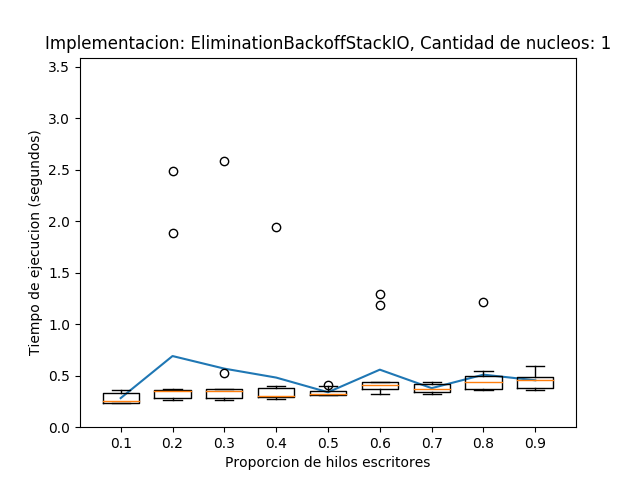
\includegraphics[width=\textwidth]{images/pushPercentages/plots/expEBSIO-1}
        \caption{Resultados para EBS sobre IO}
        \label{subfig:pushPercentages-ebsio-1}
    \end{subfigure}
    ~
    \begin{subfigure}[b]{0.49\textwidth}
        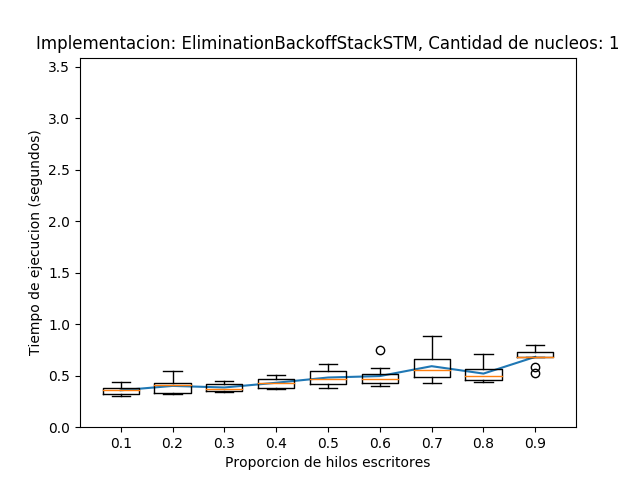
\includegraphics[width=\textwidth]{images/pushPercentages/plots/expEBSSTM-1}
        \caption{Resultados para EBS sobre STM}
        \label{subfig:pushPercentages-ebsstm-1}
    \end{subfigure}
    \begin{subfigure}[b]{0.49\textwidth}
        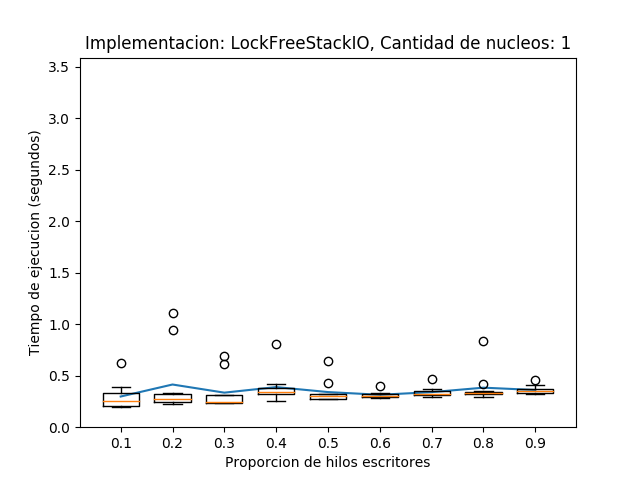
\includegraphics[width=\textwidth]{images/pushPercentages/plots/expLFSIO-1}
        \caption{Resultados para LFS sobre IO}
        \label{subfig:pushPercentages-lfsio-1}
    \end{subfigure}
    ~
    \begin{subfigure}[b]{0.49\textwidth}
        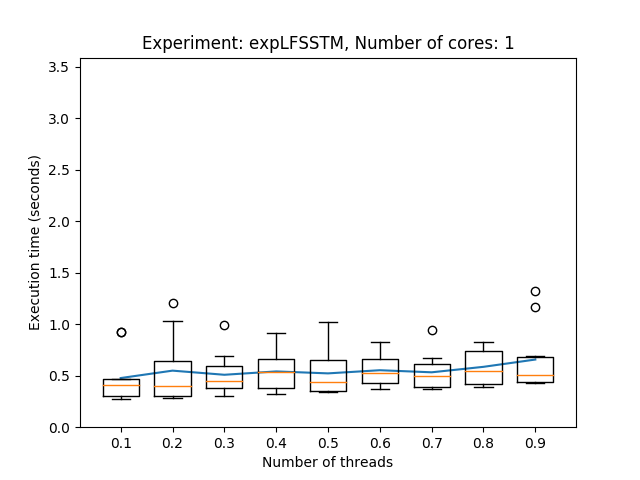
\includegraphics[width=\textwidth]{images/pushPercentages/plots/expLFSSTM-1}
        \caption{Resultados para LFS sobre STM}
        \label{subfig:pushPercentages-lfsstm-1}
    \end{subfigure}
    \begin{subfigure}[b]{0.49\textwidth}
        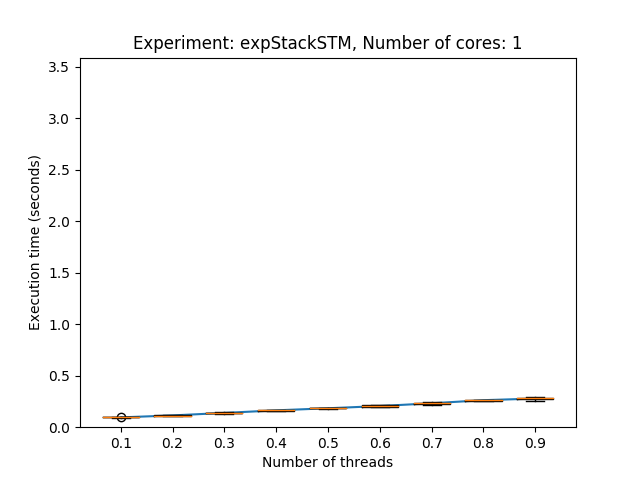
\includegraphics[width=\textwidth]{images/pushPercentages/plots/expStackSTM-1}
        \caption{Resultados para LFS sobre STM}
        \label{subfig:pushPercentages-stackstm-1}
    \end{subfigure}
    \caption{Comparación de implementaciones IO vs STM del experimento \mintinline{haskell}{pushPercentages} (1 núcleo de ejecución)}
    \label{fig:pushPercentages-boxplots-1}
\end{figure}

\begin{figure}[H]
    \centering
    \begin{subfigure}[b]{0.49\textwidth}
        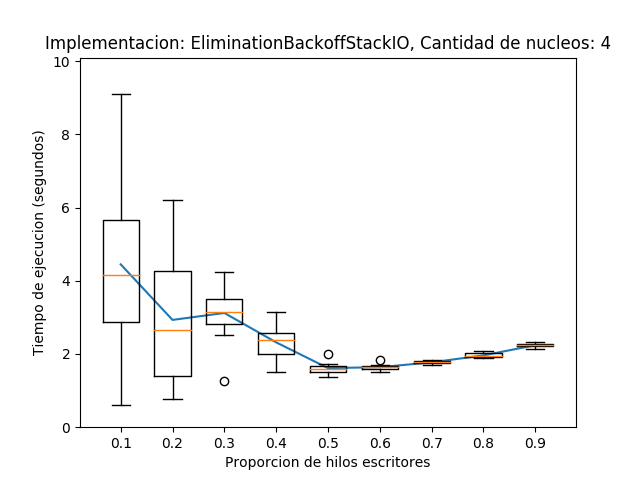
\includegraphics[width=\textwidth]{images/pushPercentages/plots/expEBSIO-4}
        \caption{Resultados para EBS sobre IO}
        \label{subfig:pushPercentages-ebsio-4}
    \end{subfigure}
    ~
    \begin{subfigure}[b]{0.49\textwidth}
        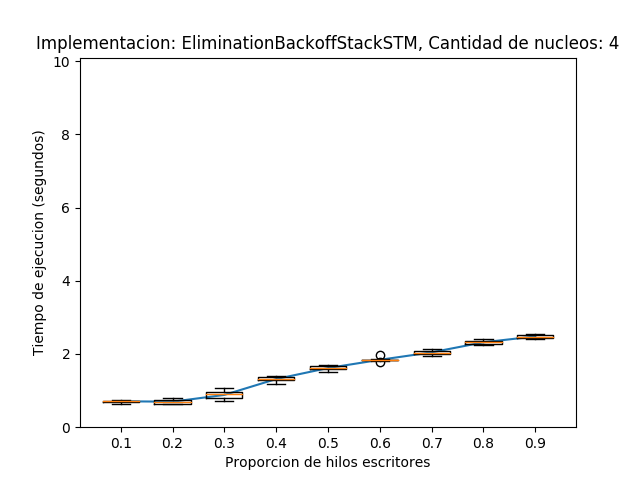
\includegraphics[width=\textwidth]{images/pushPercentages/plots/expEBSSTM-4}
        \caption{Resultados para EBS sobre STM}
        \label{subfig:pushPercentages-ebsstm-4}
    \end{subfigure}
    \begin{subfigure}[b]{0.49\textwidth}
        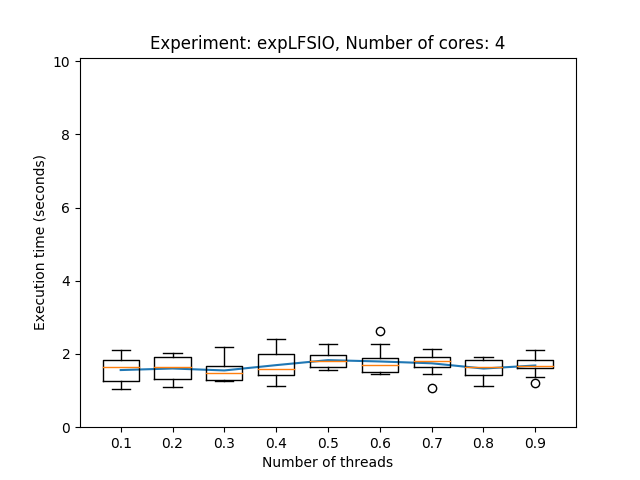
\includegraphics[width=\textwidth]{images/pushPercentages/plots/expLFSIO-4}
        \caption{Resultados para LFS sobre IO}
        \label{subfig:pushPercentages-lfsio-4}
    \end{subfigure}
    ~
    \begin{subfigure}[b]{0.49\textwidth}
        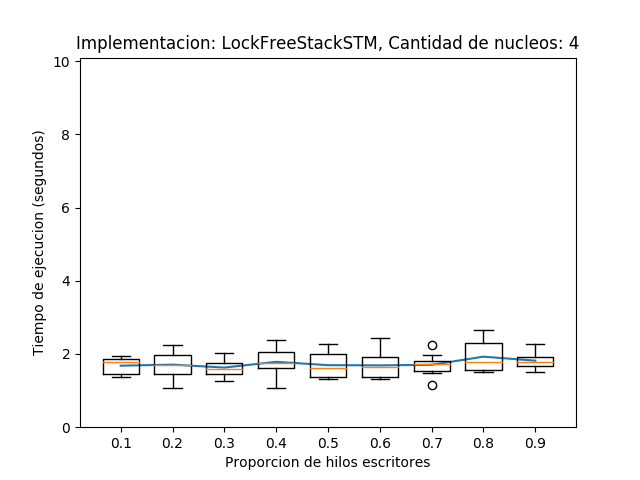
\includegraphics[width=\textwidth]{images/pushPercentages/plots/expLFSSTM-4}
        \caption{Resultados para LFS sobre STM}
        \label{subfig:pushPercentages-lfsstm-4}
    \end{subfigure}
    \begin{subfigure}[b]{0.49\textwidth}
        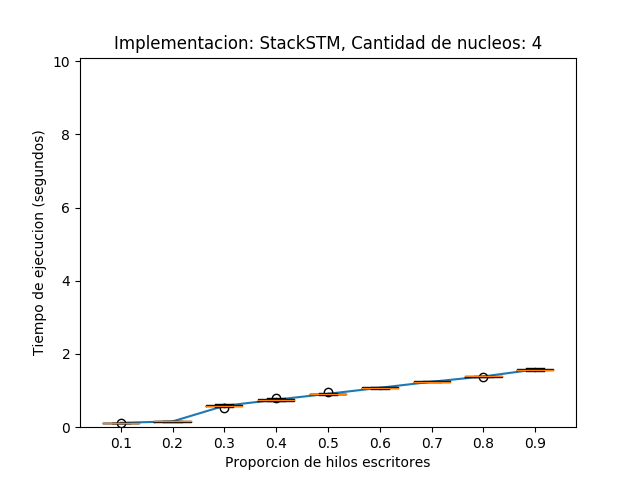
\includegraphics[width=\textwidth]{images/pushPercentages/plots/expStackSTM-4}
        \caption{Resultados para LFS sobre STM}
        \label{subfig:pushPercentages-stackstm-4}
    \end{subfigure}
    \caption{Comparación de implementaciones IO vs STM del experimento \mintinline{haskell}{pushPercentages} (4 núcleos de ejecución)}
    \label{fig:pushPercentages-boxplots-4}
\end{figure}

\section{Experimento \texttt{numberOfThreads}}
\begin{figure}[H]
    \centering
    \begin{subfigure}[b]{0.49\textwidth}
        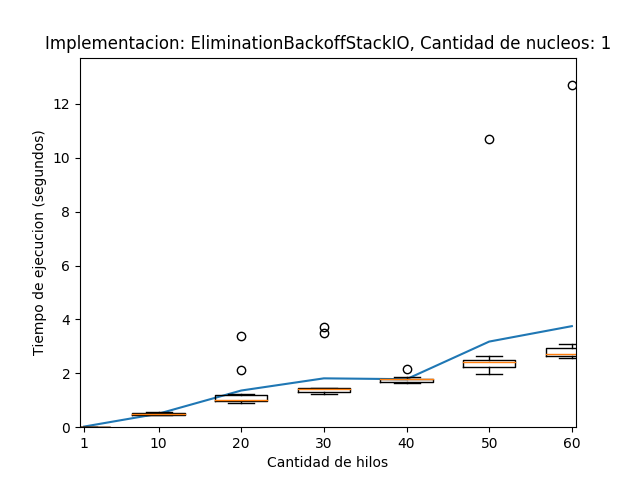
\includegraphics[width=\textwidth]{images/numberOfThreads/plots/expEBSIO-1}
        \caption{Resultados para EBS sobre IO}
        \label{subfig:numberOfThreads-ebsio-1}
    \end{subfigure}
    ~
    \begin{subfigure}[b]{0.49\textwidth}
        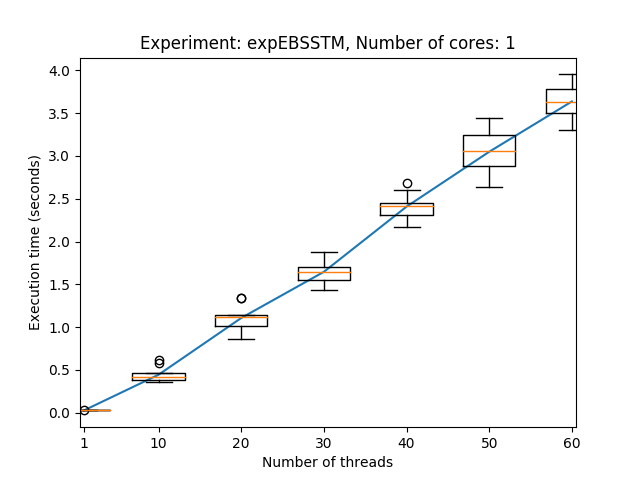
\includegraphics[width=\textwidth]{images/numberOfThreads/plots/expEBSSTM-1}
        \caption{Resultados para EBS sobre STM}
        \label{subfig:numberOfThreads-ebsstm-1}
    \end{subfigure}
    \begin{subfigure}[b]{0.49\textwidth}
        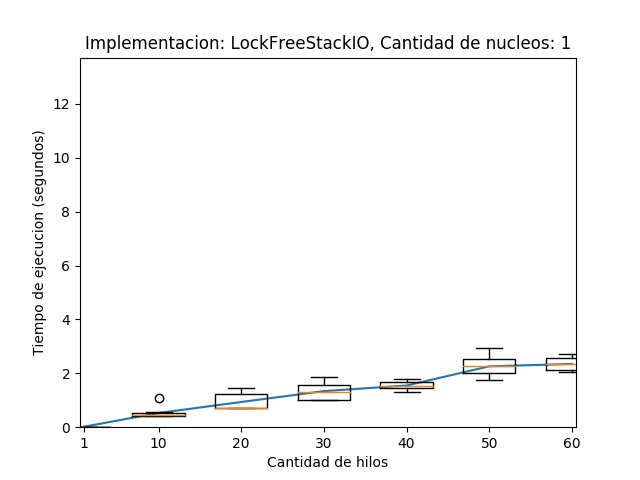
\includegraphics[width=\textwidth]{images/numberOfThreads/plots/expLFSIO-1}
        \caption{Resultados para LFS sobre IO}
        \label{subfig:numberOfThreads-lfsio-1}
    \end{subfigure}
    ~
    \begin{subfigure}[b]{0.49\textwidth}
        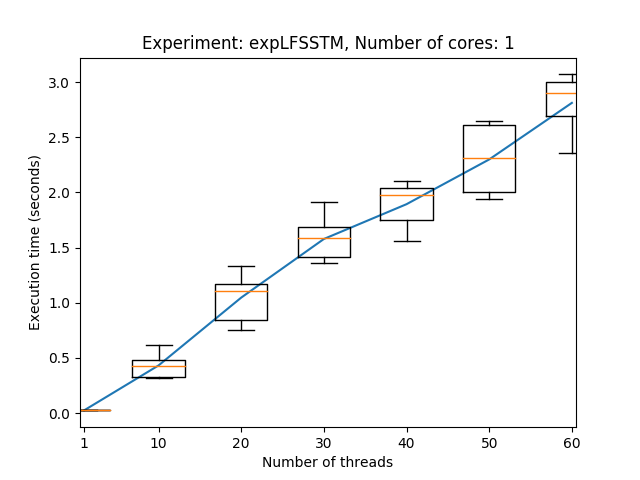
\includegraphics[width=\textwidth]{images/numberOfThreads/plots/expLFSSTM-1}
        \caption{Resultados para LFS sobre STM}
        \label{subfig:numberOfThreads-lfsstm-1}
    \end{subfigure}
    \begin{subfigure}[b]{0.49\textwidth}
        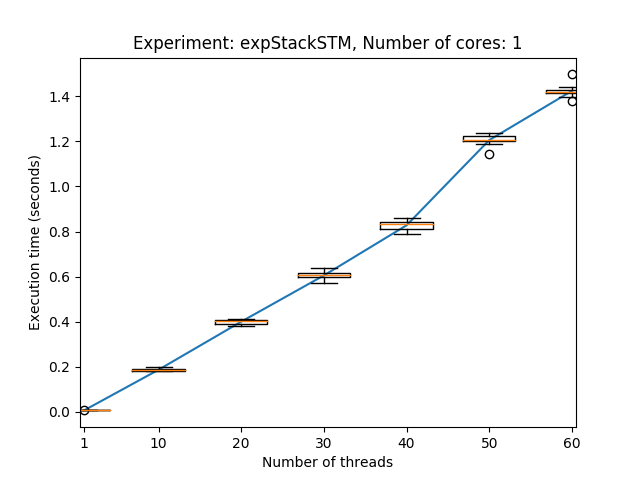
\includegraphics[width=\textwidth]{images/numberOfThreads/plots/expStackSTM-1}
        \caption{Resultados para LFS sobre STM}
        \label{subfig:numberOfThreads-stackstm-1}
    \end{subfigure}
    \caption{Comparación de implementaciones IO vs STM del experimento \mintinline{haskell}{numberOfThreads} (1 núcleo de ejecución)}
    \label{fig:numberOfThreads-boxplots-1}
\end{figure}

\begin{figure}[H]
    \centering
    \begin{subfigure}[b]{0.49\textwidth}
        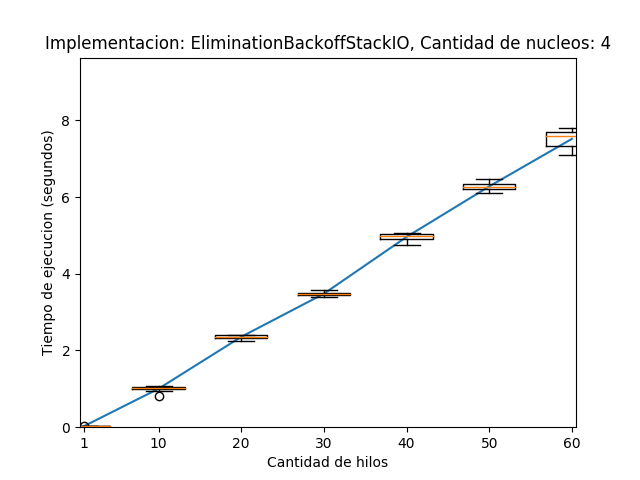
\includegraphics[width=\textwidth]{images/numberOfThreads/plots/expEBSIO-4}
        \caption{Resultados para EBS sobre IO}
        \label{subfig:numberOfThreads-ebsio-4}
    \end{subfigure}
    ~
    \begin{subfigure}[b]{0.49\textwidth}
        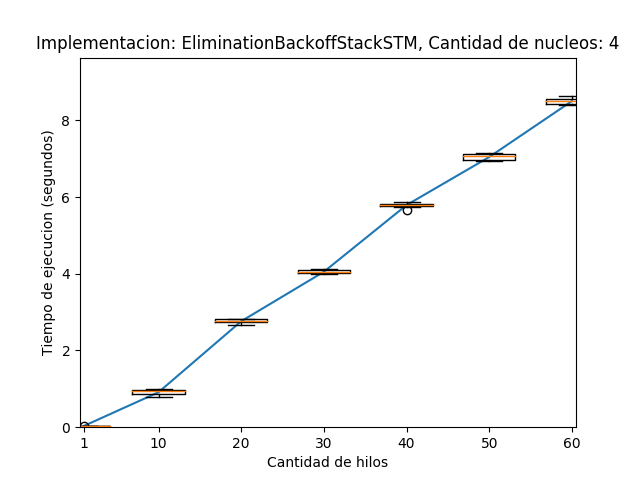
\includegraphics[width=\textwidth]{images/numberOfThreads/plots/expEBSSTM-4}
        \caption{Resultados para EBS sobre STM}
        \label{subfig:numberOfThreads-ebsstm-4}
    \end{subfigure}
    \begin{subfigure}[b]{0.49\textwidth}
        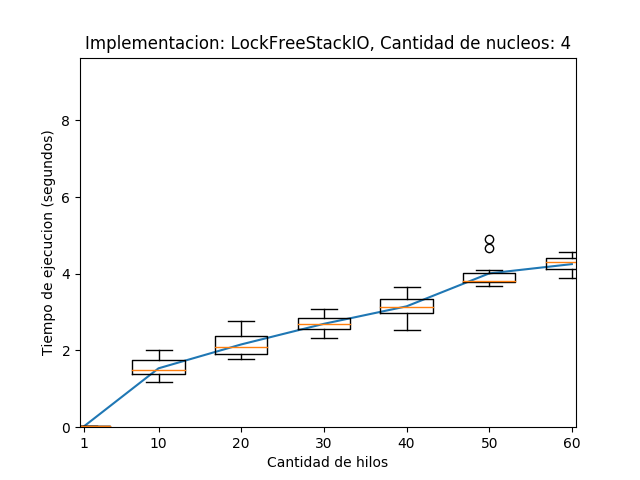
\includegraphics[width=\textwidth]{images/numberOfThreads/plots/expLFSIO-4}
        \caption{Resultados para LFS sobre IO}
        \label{subfig:numberOfThreads-lfsio-4}
    \end{subfigure}
    ~
    \begin{subfigure}[b]{0.49\textwidth}
        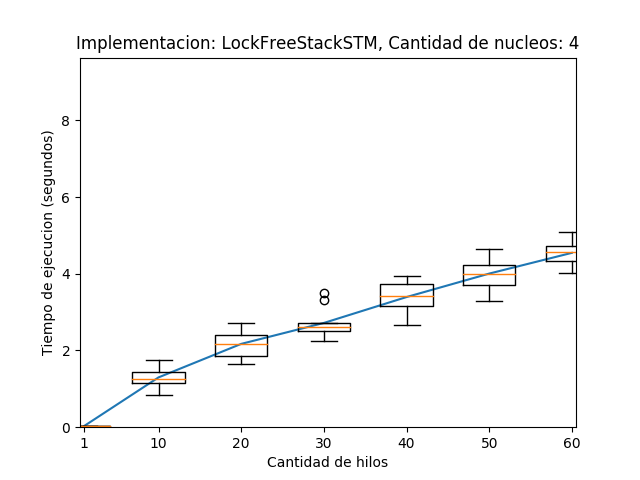
\includegraphics[width=\textwidth]{images/numberOfThreads/plots/expLFSSTM-4}
        \caption{Resultados para LFS sobre STM}
        \label{subfig:numberOfThreads-lfsstm-4}
    \end{subfigure}
    \begin{subfigure}[b]{0.49\textwidth}
        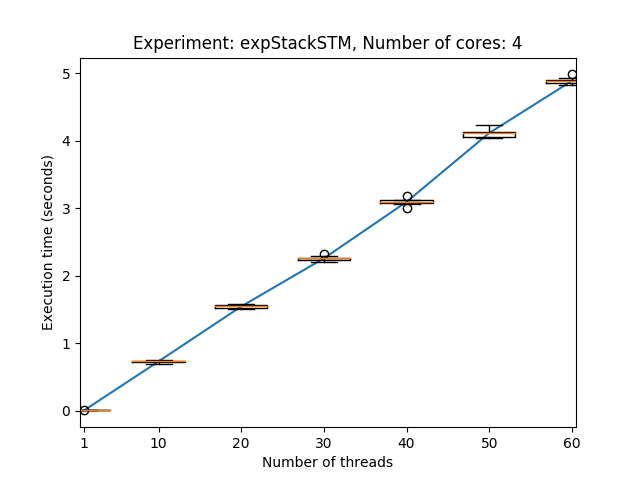
\includegraphics[width=\textwidth]{images/numberOfThreads/plots/expStackSTM-4}
        \caption{Resultados para LFS sobre STM}
        \label{subfig:numberOfThreads-stackstm-4}
    \end{subfigure}
    \caption{Comparación de implementaciones IO vs STM del experimento \mintinline{haskell}{numberOfThreads} (4 núcleos de ejecución)}
    \label{fig:numberOfThreads-boxplots-4}
\end{figure}


\section{Experimento \texttt{numberOfThreadsDist}}

\begin{figure}[H]
    \centering
    \begin{subfigure}[b]{0.49\textwidth}
        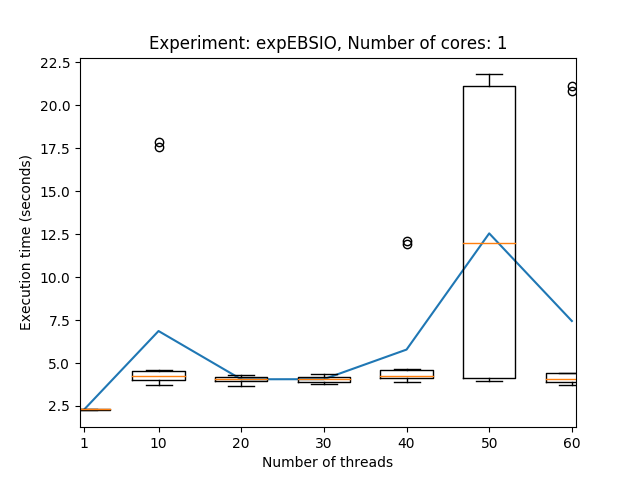
\includegraphics[width=\textwidth]{images/numberOfThreadsDist/plots/expEBSIO-1}
        \caption{Resultados para EBS sobre IO}
        \label{subfig:numberOfThreadsDist-ebsio-1}
    \end{subfigure}
    ~
    \begin{subfigure}[b]{0.49\textwidth}
        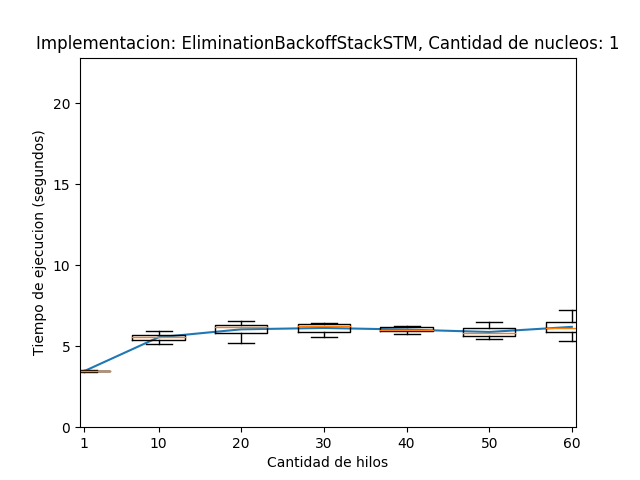
\includegraphics[width=\textwidth]{images/numberOfThreadsDist/plots/expEBSSTM-1}
        \caption{Resultados para EBS sobre STM}
        \label{subfig:numberOfThreadsDist-ebsstm-1}
    \end{subfigure}
    \begin{subfigure}[b]{0.49\textwidth}
        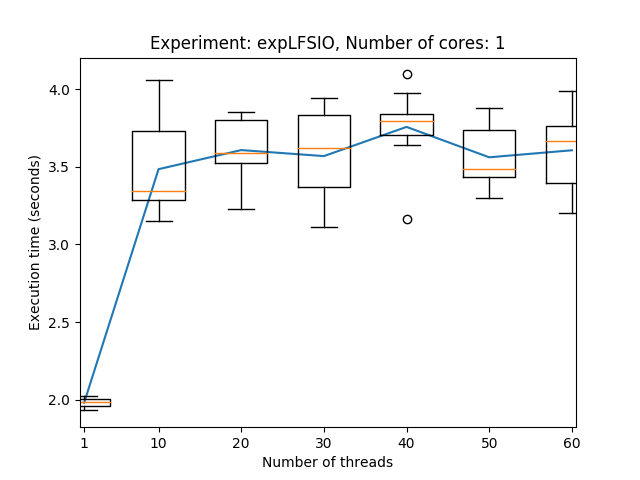
\includegraphics[width=\textwidth]{images/numberOfThreadsDist/plots/expLFSIO-1}
        \caption{Resultados para LFS sobre IO}
        \label{subfig:numberOfThreadsDist-lfsio-1}
    \end{subfigure}
    ~
    \begin{subfigure}[b]{0.49\textwidth}
        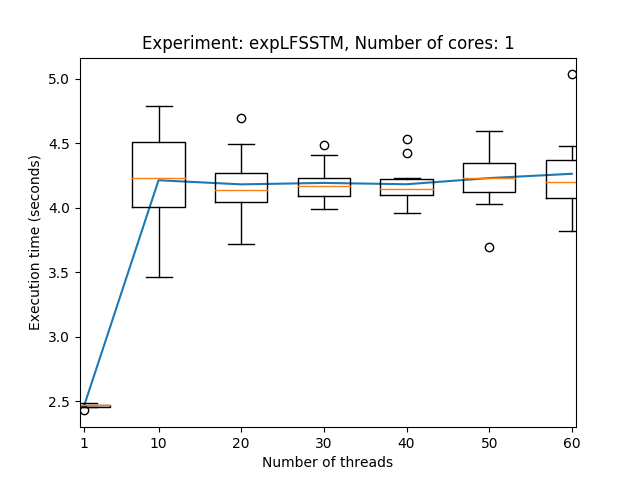
\includegraphics[width=\textwidth]{images/numberOfThreadsDist/plots/expLFSSTM-1}
        \caption{Resultados para LFS sobre STM}
        \label{subfig:numberOfThreadsDist-lfsstm-1}
    \end{subfigure}
    \begin{subfigure}[b]{0.49\textwidth}
        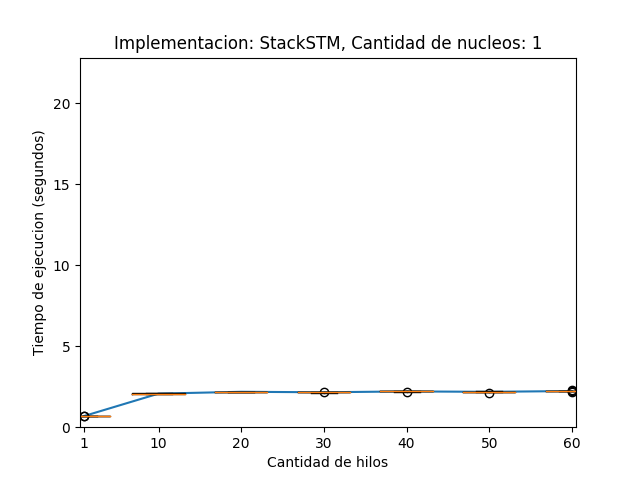
\includegraphics[width=\textwidth]{images/numberOfThreadsDist/plots/expStackSTM-1}
        \caption{Resultados para LFS sobre STM}
        \label{subfig:numberOfThreadsDist-stackstm-1}
    \end{subfigure}
    \caption{Comparación de implementaciones IO vs STM del experimento \mintinline{haskell}{numberOfThreadsDist} (1 núcleo de ejecución)}
    \label{fig:numberOfThreadsDist-boxplots-1}
\end{figure}

\begin{figure}[H]
    \centering
    \begin{subfigure}[b]{0.49\textwidth}
        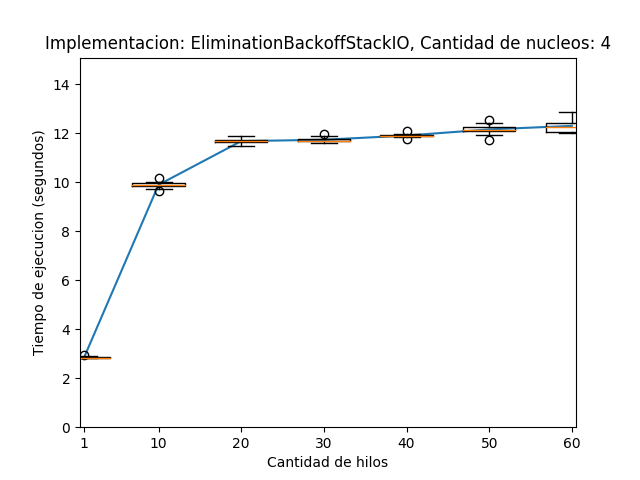
\includegraphics[width=\textwidth]{images/numberOfThreadsDist/plots/expEBSIO-4}
        \caption{Resultados para EBS sobre IO}
        \label{subfig:numberOfThreadsDist-ebsio-4}
    \end{subfigure}
    ~
    \begin{subfigure}[b]{0.49\textwidth}
        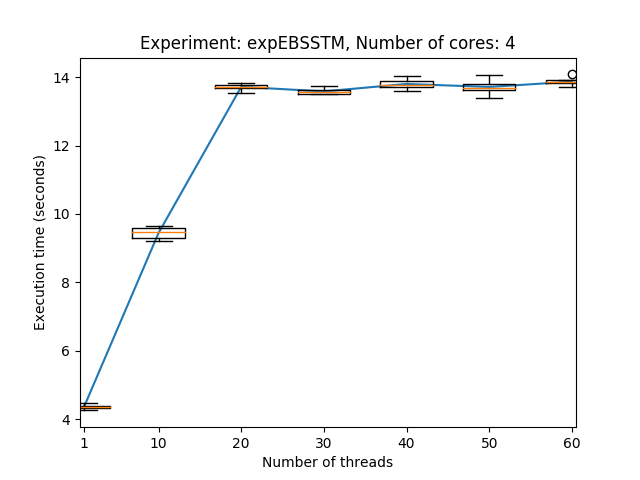
\includegraphics[width=\textwidth]{images/numberOfThreadsDist/plots/expEBSSTM-4}
        \caption{Resultados para EBS sobre STM}
        \label{subfig:numberOfThreadsDist-ebsstm-4}
    \end{subfigure}
    \begin{subfigure}[b]{0.49\textwidth}
        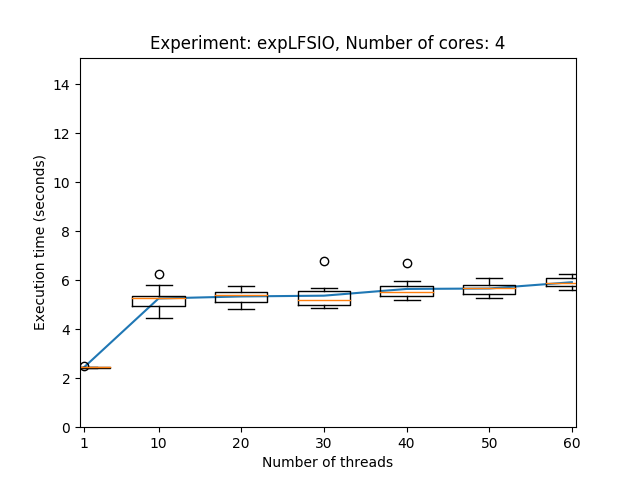
\includegraphics[width=\textwidth]{images/numberOfThreadsDist/plots/expLFSIO-4}
        \caption{Resultados para LFS sobre IO}
        \label{subfig:numberOfThreadsDist-lfsio-4}
    \end{subfigure}
    ~
    \begin{subfigure}[b]{0.49\textwidth}
        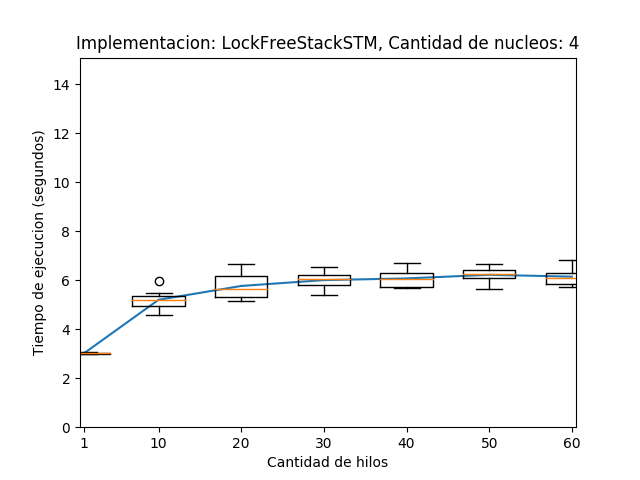
\includegraphics[width=\textwidth]{images/numberOfThreadsDist/plots/expLFSSTM-4}
        \caption{Resultados para LFS sobre STM}
        \label{subfig:numberOfThreadsDist-lfsstm-4}
    \end{subfigure}
    \begin{subfigure}[b]{0.49\textwidth}
        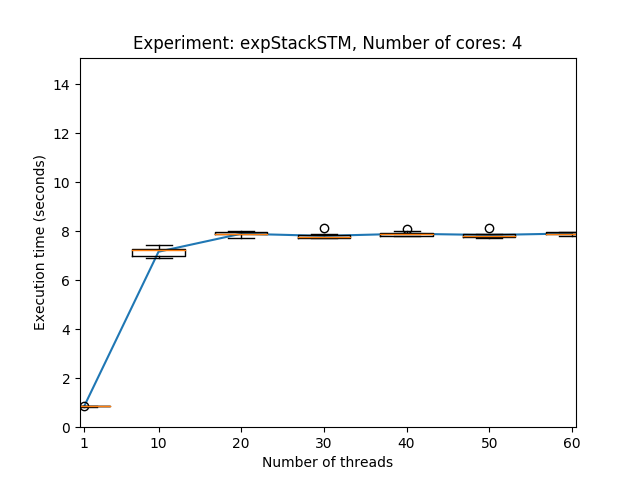
\includegraphics[width=\textwidth]{images/numberOfThreadsDist/plots/expStackSTM-4}
        \caption{Resultados para LFS sobre STM}
        \label{subfig:numberOfThreadsDist-stackstm-4}
    \end{subfigure}
    \caption{Comparación de implementaciones IO vs STM del experimento \mintinline{haskell}{numberOfThreadsDist} (4 núcleos de ejecución)}
    \label{fig:numberOfThreadsDist-boxplots-4}
\end{figure}

\end{appendices}